\begin{figure}[t!]
    \centering
    \begin{subfigure}[t]{0.23\textwidth}  
        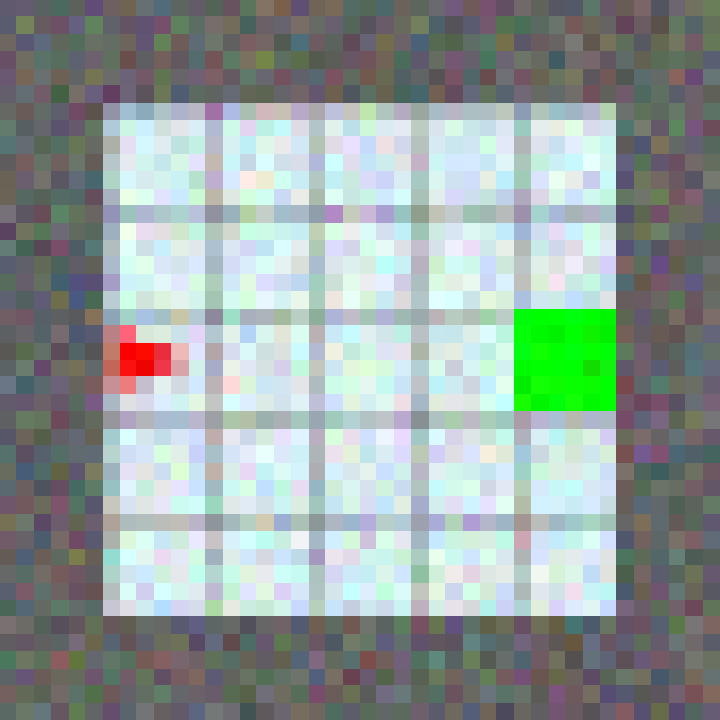
\includegraphics[width=0.49\textwidth]{figures/sec4/MiniGrid-LavaGapS7-v0_observe.pdf}  
        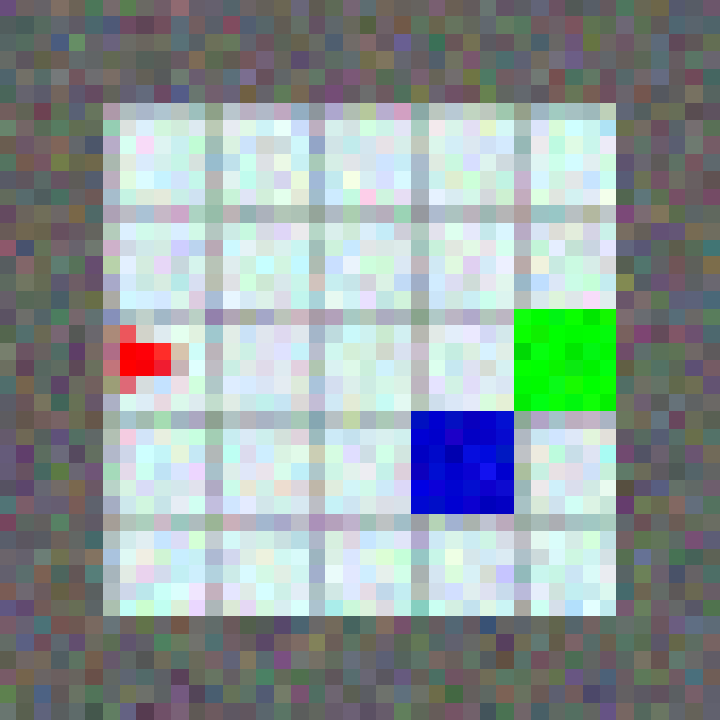
\includegraphics[width=0.49\textwidth]{figures/sec4/MiniGrid-LavaGapS7-v0_full_observe.pdf} 
        \caption{Frozen Lake.}
        \label{fig:gridworld_asym:IceLake:im}
    \end{subfigure}\hfill%
    \begin{subfigure}[t]{0.23\textwidth}  
        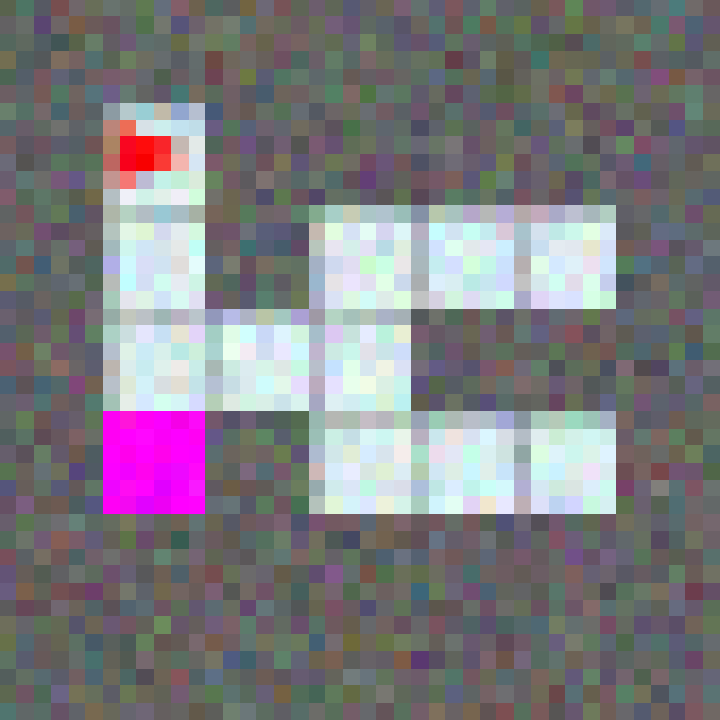
\includegraphics[width=0.49\textwidth]{figures/sec4/MiniGrid-TigerDoorEnv-v0_observe.pdf}
        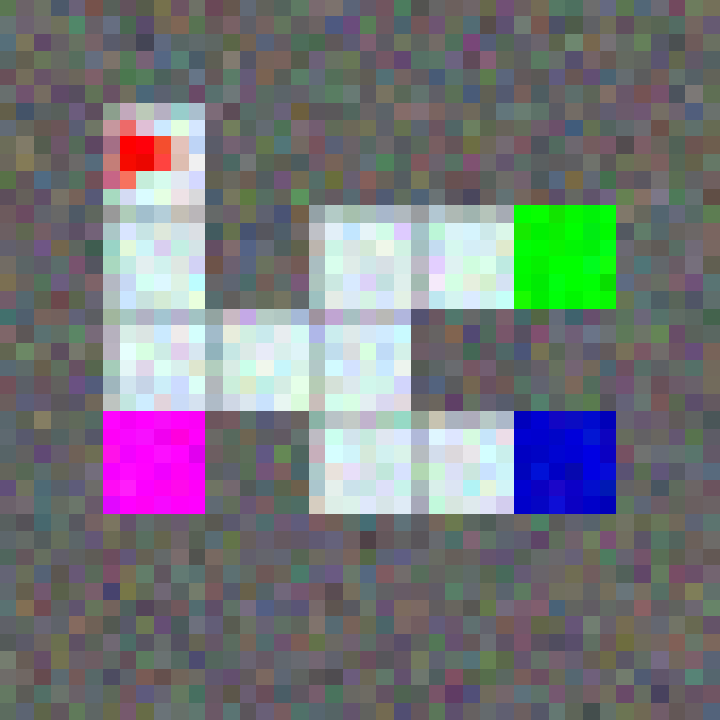
\includegraphics[width=0.49\textwidth]{figures/sec4/MiniGrid-TigerDoorEnv-v0_full_observe.pdf} 
        \caption{Tiger Door.}
        \label{fig:gridworld_asym:TigerDoor:im}
    \end{subfigure}
    \caption{The two gridworlds we study.  An agent (red) must navigate to the goal (green) while avoiding the hazard (blue).  Shown are the raw, noisy $42\times 42$ pixel observations available to the agent.  The expert is conditioned on an omniscient compact state vector indicating the position of the goal and hazard.  In Frozen Lake, the trainee is conditioned on the left image and cannot see the hazard.  In Tiger Door, pushing the button (pink) illuminates the hazard.  } 
    \label{fig:gridworld_asym:grids}
\end{figure}
